\section{实现原理}
\subsection{不同的上下文的动作实现}
在软件当中,通常要实现这样的操作,比如主窗口内有很多的控件,每一个控件可能都有自己对应的复制粘贴删除的动作,按下相应的快捷键之后,如何判断现在是属于哪个控件,应该执行哪个控件对应的命令。

我按下del键,有可能是删除文件,也有可能是删除图形,如何进行相应的判断?

\subsection{工程树当中的数据保存问题}
在Qt当中,树形控件是采用视图模型委托的设计模式,也就是,你需要自定义对应的抽象类文件,实现子类。Qt已经实现好了数据读取,设置的函数模版,你只需要重新根据你的需要进行实现即可。自由度最大的就是真实数据的保存,很明显,传递给树控件的数据和真实的数据还是应该分离的。那么真实的数据应该保存在什么位置?project的类变量当中?毕竟这是属于这个项目的。那么新的问题就来了,需要更多的新的数据类型,比如你要自定义变量类型吧,然后你在project当中保存一个变量的list或者map。你还要实现材料,几何,分网,还有一堆杂七杂八的东西。你需要监控这些变量的改变,然后对应的更新树控件当中的node显示,反过来也是一样的,如果对node进行了相应的修改操作,那么就需要更新对应的变量。问题是,采用什么样的方法进行更新呢?应该是在修改后直接更新吧。

如何将node的数据与真实的数据关联起来?
\subsection{Node的设计问题}
工程树当中有很多的node,不光是数量多,而且种类也非常的多。应该如何设计它的继承关系?比较纠结的就是一个node类型目前设置的是没有子节点的,所以它应该是直接从顶层node继承过来的,如果以后想要更改功能,给它添加子节点,那就要再次修改它的继承关系啊。
\subsection{动作的管理}
在一个大型的软件当中,必然会有数不清的actions,而且在一个类当中可能要去调用另外一个类的action,所以就需要一种策略来将所有的actions集中存储起来。集中存储的话避免不了前面说的一个问题,相同的动作ID。

现在知道了应该创建一个map或者hash类型的变量来保存变量,并实现检索。hash的好处就是搜索速度能够快点儿。但是,由于现在采用的不是菜单风格,ribbon式的UI它不光可以添加action,它还可以添加widget,这样留出接口就比较麻烦了吧。
\subsection{材料树}
材料树跟工程树不太一样,因为里面只包含材料,多一点的可能就是材料的分类,这个就相当于是一个容器或者文件夹。

有一种想法,材料的确是一个大类,非常复杂,但是,当我们去查询某个材料的某个属性的时候,就像是查询数据库一样的,它有那个材料属性的名字,然后对应的有一个单位和数值。所以,想要将材料设计的更加丰富,可以将其抽象为属性的集合,这些属性从属于不同的分类和学科,也有可能只存在于某些条件下,只在特定的情形才会有这个属性。这样的设计,材料可简单,可复杂。其实,在设计软件的时候,并不是不能找到一种解决方案,而是,太不容易开始,又太容易考虑太多的未来的东西而缚手缚脚。你写得东西要给别人用,要一直用,要给更多的模块用,
\subsection{代数模块}
需要很好的定义一些代数模型,并保证不随便更改。包含矩阵,向量,线性操作。当然要注重性能和实用性。稳妥的方式就是采用现成的模块。
\subsection{多边形填充}
联想一下,多边形“回”字填充网上没搜到什么有用的东西,那就换一个思路,圆环是一个很常见的图形,比如圆环形状的进度条,这个总要填充吧,这个网上总有资料吧?查了一下果然有,绘制环形填充的方法,有的人就有用遮罩的方式,不过这种方法在有的时候就会露馅,不太推荐。另外一种方式就是采用QPainterPath这个类,它可以添加各种的路径,然后在各个路径之间进行填充,验证了一下,发现好使。
\begin{figure}[htbp]
	\centering
	\subfigure[CAD模型]{
	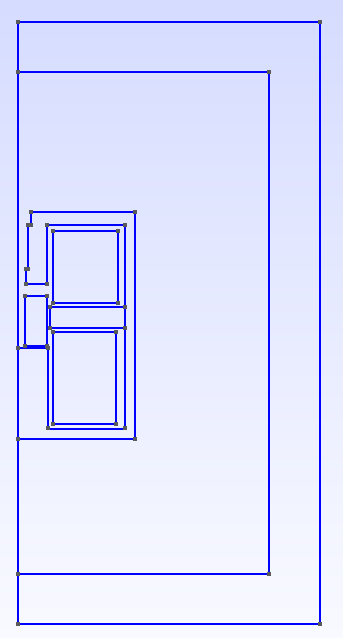
\includegraphics[width=0.35 \linewidth]{figures/model.png}
	\label{fig:model}
	}
	\hspace{0.16 \linewidth}
	\subfigure[Qt实现填充区域]{
	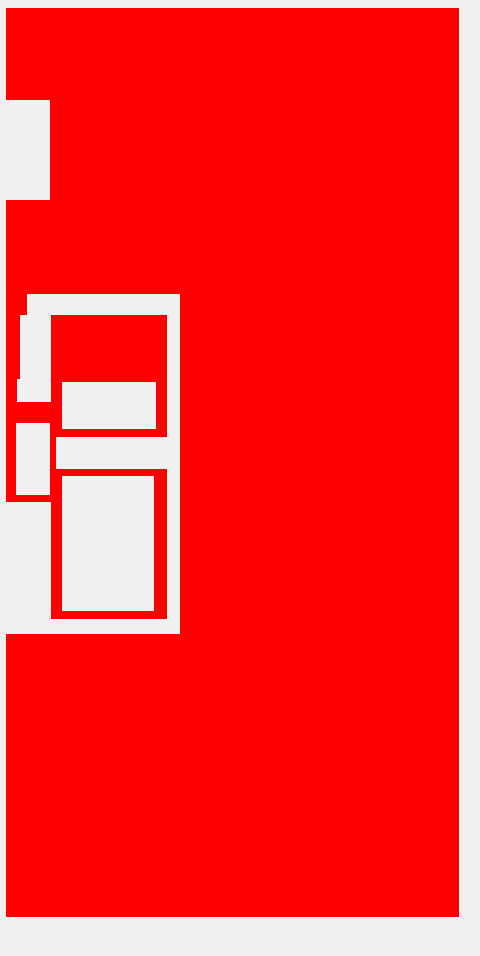
\includegraphics[width=0.33 \linewidth]{figures/path1.png}
	\label{fig:path1}
	}
	\caption{CAD模型以及空气区域的填充效果}
\end{figure}
然后令人比较惊奇的是,这个类还可以检测点是否在路径的内部,虽然并没有搞懂绘制路径的原理,但是莫名的好使,需要进一步研究路径的原理来使用它。

在填充路径时要用到填充规则,这里一共有两个填充规则

path.setFillRule(Qt::OddEvenFill);//奇偶填充规则

如果要判断一个点是否在图形中,可以从该点向图形外引一条水平线,如果该水平线与图形的交点人个数为奇数,那么该点在在图形中。

只填充在图形内的点

path.setFillRule(Qt::WindingFill); //非零弯曲规则

如果要判断一个点是否在图形中,可以从该点向图形外引一条水平线,如果该水平线与图形的边线相交,这个边线是顺时针绘制的,就记为1,是逆时针绘制的就记为-1,然后将所有数值相加,结果不为0,那么该点就在图形中。

QPainterPath判断点在内部的算法:

1.检查path是否为空,点是否在path的边界内;

2.根据path当中的元素进行迭代;

3.针对每一个path,按照上面的方法,做一条水平线,计算交点的个数,最后统计交点的总数,如果是奇偶填充规则的话,偶数就代表不在区域内部,不填充;奇数代表在区域内,填充;如果是windingfill,就判断曲线的逆时针和顺时针的方向,最后求和是不是0。

但是,具体填充的是否不会是这样判断的吧,如果是这样的话,计算量有点大啊。
\subsection{建立face}
可以简单的建立face,保存数据并不困难,难的是怎样把face绘制出来。一般的face的话,采用填充就可以了,但是对于有嵌套的face,填充就不好使了,可以想到的办法就是使用qt当中的path来绘制,它的绘制原理是按照奇偶填充绘制的,能够实现所想要的效果。
\subsection{如何保存tree的展开状态?}
应该是要保存哪些节点需要展开,哪些节点需要折叠。
\subsection{关于单元建模}
主要纠结的地方在于,单元的保存格式跟几何形状的保存格式并不一样,如果单纯的按照一方来保存,是不是过于强耦合?现在的逐步的感觉难度在于建模方面,你要考虑有限元当中的模型,cad的模型,绘图的模型,还有求解的线性代数的模型,每一个都需要有实际的经验来进行设计,不一定你设计的就是最好的,但是一定得是有道理的,主流的方法。
\subsection{如何使用gmsh的链接库?}
如果能够使用gmsh的链接库,那么就可以使用其中的大量的api进行操作,就不比只使用exe操作有用的多。


\subsubsection{插件如何翻译}
目前还是在一个文件里进行翻译,好像没什么能够合并的方法。
\subsection{模型传递的问题}
鉴于传入到求解器当中的参数很多,

\subsection{复杂几何模型问题}
很明显,将过多的精力放在并不擅长或者永远见不到头的CAD上面是不够明智的,只需要满足最基本的需求即可,过多的功能无需实现,也没有必要实现,COMSOL也不见得能够建立多么复杂的模型,退而求其次的方法就是具备几何模型导入和分网导入功能,这样对开发进度是一个很好的解脱。
\subsection{坐标系的种类}
常见的坐标系有:笛卡尔坐标系(也就是直角坐标系),圆柱坐标系,极坐标系。根据对称性来分类,无对称,有对称面,有对称轴。
\subsection{如何设计solver的位置?}
求解器,准确的来说只是一个求解的函数,但是如何进行合理的设计,利用好cpp的类的设计风格?感觉c当中的那种纯函数的风格更加的不错,可以直接调用。其实cpp的类当中不一定需要设计成员变量,可以出现没有成员变量,只有函数的情况,也可以存在只有成员变量,没有函数的情况。但是,其实后一种编译器会自动的添加默认的构造函数和析构函数,同时,也要求你的类成员变量需要有默认的构造函数,否则编译器就无法调用准确的构造函数完成初始化任务。
\subsection{有限元装配原理}
在大多数的有限元求解当中,是需要矩阵装配过程的。也就是将有限元的单元矩阵合成为全局矩阵,然后进行后续的迭代求解。根据矩阵的格式,可以分为全矩阵和稀疏矩阵两种格式。如果是全矩阵的话,装配过程就相对比较简单,只需要将矩阵元素跟全矩阵对应位置的元素相加即可。如果是稀疏矩阵,最后生成的格式是对应的稀疏格式,装配起来就会复杂一些。具体的可以参考文件SpMat\_meat.hpp。

我觉得生成的思路有好几种,一种是直接生成的,将所有非零元素的值和位置进行保存,由于同一个位置可能有多个相加值,然后需要计算出每一个位置的相加后的值,得到位置与非零值的对应数组,最后就是将数组进行压缩,就得到稀疏矩阵的保存格式。

另外一种方法就是,使用死办法先创建一个全矩阵,然后将装配结果保存到这个矩阵当中,全矩阵的好处就是检索比较方便。由于全矩阵很占内存,最后再将所有的0去除,得到非零元素,最后再得到压缩后的稀疏矩阵格式。
\subsection{细节}
最不缺少的是流程图和框图。因为上面等于什么也没说,想要实现的话还得看细节。大家都知道步骤A之后是步骤B,但是问题就是如何过渡过去的事情。接口这事情,没有经验,最开始是写不不好的,还不如先不写,最后需要扩充的时候再写。
\subsection{捕捉实体}
为了实现实体形状的选择,就要依靠鼠标指针的位置来判断是否在形状的范围内。看上去似乎很不错,但是有一个问题,有些形状是最基本的,不可以分割的,而有一些形状就是由其他形状拼接过来的,比如矩形就是四条直线拼成的。那为什么不让矩形不可拆分呢?
\subsection{filelistchanged}
采用信号槽的方法来动态的更新列表。主要是要对那几个顶部的node进行操作。

Project::handleSubTreeChanged -> ProjectTree::emitSubtreeChanged -> ProjectTree::subtreeChanged -> FlatModel::updateSubtree -> FlatModel::addOrRebuildProjectModel

对于树的更新,有两个方面,一个是刚开始的时候创建了一个project,这个时候需要添加一个项目添加的处理,就要build一下project,这个是一个信号,就是添加项目,然后我自己修改tree的话,就不再是添加了,而是tree的改变了。tree的改变也是一个信号,也需要调用rebuild的操作,那是如何保证不改变原来的部分呢?就是每一个项目的根节点,它对应的都是一个项目,在改变tree的时候,先要找到project对应的根节点,然后把它的所有的children给清空,然后在这之前你需要更新一下projectnode,然后就可以把projectnode添加为到treeitem。所以,问题就在于,如果更新了node,之后,就需要重新生成projectnode。

现在终于看懂了,主要有两条线,一条是node,另外一条是treeitem。其实之前主要忧虑的地方在于移动之后,node还在不在了,移动之后,指针的指向还是正确的,只不过不再属于原来的变量了。由于node的保存是树状的,最后都会跑到顶部节点下面,还是只能能够检索到子节点,还是能够正常访问的,内存并没有被释放,数据也没有丢失。这是project的node列表。为了能够在控件上显示树列表,就要把node转化为model当中的treeitem数据,这个也是按照树结构保存的,所以只要调用递归函数进行生成就可以了。model就可以自动的根据调用函数来读取所有的items。然后其他的编辑访问操作,都是最后读取到对应的node。为了添加或者删除node,先是要通过tree获得当前选中的节点,然后对该节点进行操作就可以了,然后发射树改变的信号,就能实现tree的改变。

我成功地按照这种方法添加了子节点,但是,需要弹出对话框来设置材料,要是能够获得dialog的执行结果就好了。这样就能进行判断。每一个对话框会返回accept结果或者reject结果。

我可以寻找各个标志所在的node,
\subsection{对话框的创建}
在软件的运行过程当中,肯定会有很多的对话框出现,应当以ui的方式建立窗体还是以代码的方式建立窗体?还有,如何批量的建立窗体。

从功能上讲,ui和代码设计都能达到相同的效果,当然,代码的能力可能会更强大一些。
\subsection{创建tree的右键菜单}
1.先在actionmanager当中创建一个菜单的ActionContainer*,这个manager已经在主窗口当中进行了初始化了;

2.然后在菜单当中创建所需要的group,每一个group都代表了一类功能,group是一个特定字符串代表的值,不同的container可以含有相同的字符串,就像每栋楼都有101房间一样,默认的,为了防止将action加入到一个空的container,container自带三个group,会将没有id的action添加到这三个的其中一个;

3.接下来就是给各个group当中添加actions,在添加第一个action之前,需要添加一个分隔符,然后就是不断的添加action到对应的group了。同一个action可以添加到不同的group当中。小技巧就是,在h文件当中定义一些group的常量名称。

4.在treeview的showContextMenu函数当中,根据不同的节点类型,调用显示不同的菜单。
\subsection{如何统计代码的总行数?}
采用正则表达式进行匹配搜索,但是有误差。
\begin{lstlisting}
	b*[^:b#/]+.*
\end{lstlisting}
\subsection{armadillo中的稀疏矩阵装配过程}

\subsection{绘制方形的时候,直线不黑,严重虚化}
感觉是在坐标强制转换的时候出了错误,有的时候会差一个像素点,导致参考点绘制的时候不在中心上。而且有的时候,一条黑色的直线会画成两条,一条灰色的,一条黑色的。有的时候就没有。如图\ref{fig:linemohu}所示。
\begin{figure}
	\centering
	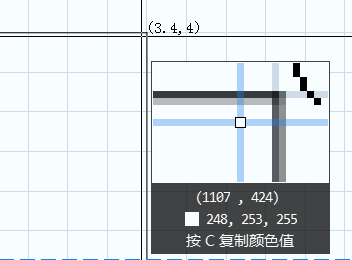
\includegraphics[width=0.7\linewidth]{figures/linemohu}
	\caption{绘制的直线不黑,模糊}
	\label{fig:linemohu}
\end{figure}
发现这并不是偶然出现的,而是确实哪里有问题。我们来查找一下原因。绘直线最基本的就是两个点,如果两个点的坐标算错了,那么画出来的图有可能因为变歪而显得模糊,因为水平和竖直线肯定总比斜线要清晰。但是经过排查,其实坐标没什么问题,虽然它使用了float类型的point,但是我觉得这不是问题所在。那问题就可能出现在绘制的过程当中。接下来不断地进行跳转到drawline函数的实现,发现在绘图之前需要判断是否要抗锯齿化,只有设置了抗锯齿化之后才会变得清晰。所以,问题就变成了确认一下在绘制直线的时候是不是抗锯齿化的,如果不是,那么这就是问题所在。发现drawline并没有被显式地设置抗锯齿化。

需要注意的是,实际的坐标值转化为像素点的时候,它不是一个整数,肯定会有小数位,然后你绘制的时候,可能就是以像素点为标准绘制的,严格意义上讲,是不准的。反过来,你捕捉点的时候,你捕捉的是像素点,然后你将像素点转化为坐标点,这个值也是不能跟实际坐标点完全对应的,肯定会有误差。需要知道qline和qlinef的区别。从文档中来看,这样做只是为了扩大坐标点的存储范围。
\subsection{treemodel是如何建立索引的?}
父索引,也就是root索引这个肯定是有的,有了这个,就可以递归的生成其它的索引了。所以,下一步就是在project当中定义model,然后在treemodel当中添加对project的处理,这样就可以了。可以先在内存当中测试,等到测试没有问题了,再添加对文件的读写。

\subsection{是如何达到效果的?}
通过反复印证。
\subsection{属性页如何实现}
需要点击树控件上的每一行,切换页面,还是qstacklayout?
\subsection{Node的设计}
主要针对于树控件当中的Node的设计。树控件是重要的交互界面。先找到问题,然后尝试在各种情景下复现问题,分析问题产生的原因,定位使问题产生的环节,最后尝试修复该环节。

没有子节点的Node可以有两种,一种是在定义实现当中没有子Node,未来也无法扩展该功能,另一种就是有子Node,但是在接口上没有实现,未来根据需要可以进一步地开发。为了避免Nodes随意的插入,是不是可以加入排序功能,将相同的Node排序到统一的节点下,但是,在某些情景下,Node之间的相互顺序是很重要的。

为了避免Node插错位置,我觉得需要在插入的时候进行类型判断,如果类型不对,就不让插入。或者,每一个node设定一个级别属性,级别低的不能插入到级别高的node下。应该是tree的列数吧,根部节点只能插入到第一列,二级节点插入到第二列。

同时,还要考虑数据存储的问题。

基类的Node。感觉这里的node之间没有什么特别明显的继承关系,都挺孤立的。

\subsection{材料库}
预先准备好材料库文件,打开对话框之前,读入文件并且显示。不同的物理问题对应的材料库应该不同。因为他们所关注的属性不一样。所以,这就给建模带来了一个问题。每一种材料的属性都要建的非常全面。
\subsection{生成树的算法}
如果存在project文件,准备文件;

分析文件;

写node。

这是针对硬盘上的数据,如果是内存当中的数据,本身不会采用文件的这种格式,而是具体的数据。总结起来,有三个数据,一个是硬盘上的,一个是节点node,一个是真实的变量。这三个应该如何权衡之间的关系?我认为大体的思路是没有错的,只不过可能比他们更加缺少对实现细节的考虑或者对功能的设计。按道理讲,三者的数据应该是同步的,一个对数据进行了修改,其余两个都要进行改变。关键在于辨别那个数据才是最新的。project最初打开,最终保存的时候,会涉及到硬盘文件存储,在整个其他的操作过程当中,可能都是在内存当中存储的。project应该和node共享变量指针。

“两年前我还在折腾Linux Kernel的时候, 正碰上他们组发表了一篇修改Linux内核的锁实现, 以在众核(单机超过32核)情况下提升应用性能的文章. 文章效果非常好, 使用的几个workload都达到了近乎线性的加速比. 我在学术讨论会上报告这篇文章的时候, 大老板听闻这篇文章只不过编写了1600+行代码, 大手一挥让我们大干快上, 也搞个类似的出来. 可是改内核这种事情, 别说修改1600行, 就是改一行代码, 想要知道在哪里修改能够取得预期的效果, 对普通的博士生来说其背后的工作量都是难以估算的. ”
\subsection{vs code and $\LaTeX$}
已经看不惯了texstudio那样丑陋的界面了,心动之下打算尝试一下vs code。首先,vs code的启动速度在新电脑上没有那么慢,而且界面风格比较喜欢,网上也有很多设置latex环境的方法,非常简单。只需要安装latex workshop的插件就可以了。还可以设置pdf的正反向搜索跳转。需要注意的是,如果使用的是sumatrapdf软件,并且是在vscode的左侧树当中打开的这个软件,那么,似乎是因为这个是属于vscode的一个进程,所以,反向跳转可能会不好使。需要单独地在外部打开软件进行跳转即可。真的是非常喜欢x1c打字的键盘。清脆。尤其是高清的屏幕看起来非常有质感。但是还不知道怎么设置正向搜索,哈哈。
\subsection{模块之间开发不同步的问题}


\subsection{有一个问题}
在开发的过程当中,发现不管是要实现的函数,要规划的任务,都实在太多了,一不小心就不知道开发到什么地步了,什么功能有没有实现,实现到什么程度了,有没有被测试,有没有bug,好不好使。应当有那样的一个任务板,设定好要实现的计划和任务,明确规定功能的详细内容以及预计完成的日期。
\subsection{插件放哪里?}
插件的声明,应该放在mainwindow当中吗?从插件的功能来看,这就不属于主窗口的东西,而是独立于它的一部分,但是由于主窗口留出了访问其内部资源的接口,所以,也不必在mainwindow中实现。

但是,这是人家插件系统当中的版本。人家是通过一个插件管理器来载入了所有的插件,进而能够访问所有的资源和功能。反正怎样写都可以实现。如果是单独开发的话,写到main当中,这样集成度更高一些,因为这本来就是自己写的,而不是第三方,所以为什么不能放进去?可以的。但是,一定要注意初始化的顺序,有些插件是依赖于别的插件的,有先后顺序之分的,不然资源还没有被创建,后面的都JJ了。
\subsection{qDebug重定位}
我有一个大胆的想法,在调试的过程当中,总是要去看qtcreator的输出信息,窗口要切换来去非常的繁琐,要是直接能够把信息定位到我的log窗口,那么就不需要切换窗口了。之所以想定位debug,是因为不想改太多的代码。

仔细地查了一下资料,实现的原理很简单,就是重新实现一个qdebug,也就是定义一个新的宏命令吧。
\subsection{绘图的交互}
在绘图的时候,是设置为必须先绘制所有的点,然后再连接得到线段,最后再生成面。还是,可以随意的绘制。

第一种的好处就是,整个图形都是由最底层的点的坐标组成的,只要修改点的坐标,整个图形就可以相应地进行更新,而另外一种,就必须对每一个图形进行修改,因为它的坐标都是内部的,与其他的没有什么联系。
\subsection{生成面的算法}
刚开始比较好奇计算机是怎样实现不规则形状多边形的填充的,就搜索了一下奇偶填充算法,真的找到了很多资料,有很多的算法。看着看着就看到了一个主题,平面内封闭区间的识别,这个问题应该与生成面的算法类似吧?看到有人提出用计算图形学当中的一个漫水填充算法,这个名字真的好形象,在区域内找一个点,然后就开始递归式的开始填充,如果没有碰到边界,就不断地向前搜索,最后所有的区域都被填充了。但是效率实在太低了,每个点都要进行判断。

但是,还是不如直接设置方便啊。数据量小的话,还是手动设置吧!
\subsection{treemodel}
qmodelindex这个变量它所指向的东西可能会变,因为它的含义是某行某列,而模型当中可能会插入一些数据,导致它的行列数已经发生了改变。但是index当中不是保存了数据的真实指针了吗?
\subsection{图形选择}
选择的实体,是要单独的保存出来呢,还是要标记为“选中”状态就可以了?按道理讲,没必要那样做。选中状态的效果,是采用了不同的笔刷来实现的,只要跟正常画的不一样,就会给人以选中的状态,因为在单击鼠标的那一刻,图形颜色改变了,有反馈说明被选中了,因为只有选中了才会有改变啊。cad并没有在每一个形状的draw函数当中单独的进行选中的判断,而是放到了graphicview当中集中处理。这样的好处就是节省代码量。

绘制图形前需要判断:
\begin{enumerate}
	\item 是否存在;
	\item 是否可见;
	\item 是否在显示区域内;
	\item 设置笔刷;
	\item 是否被选中;
\end{enumerate}
\subsection{调试}
大型软件怎么调试?光是编译有时候可能都得十几分钟,有的甚至有几小时,几天的,这种情况还整个跑起来调试不太现实吧,应该都是单个模块调试吧。
\subsection{更新}
以谁为更新依据原理应该是谁先获得焦点。

\subsection{menu}
之前在顾虑ribbon的page上的每一个group都是一个控件,没办法插入菜单。但是,似乎理解不够,抽象不够彻底。group上面的动作,可以通过添加action来实现,menu本质上也是一种widget,所以group也是可以插入menu的。
\subsection{tree与node}
还是搞不清楚之间的关系。我觉得大型软件编程有这么几个问题:第一,要有非常明确的需求,不论是怎样的幻想,设计,最后都要落实到具体的细节上,而不是简单的,我就是想要实现一个类似什么的功能,同时,也要避免后期的无端的需求变化;第二,不只是只有我有这种想法,我曾经以为计算机科学课上学过的“面向对象”是很简单的东西。我的意思是,创建一些类来模拟现实世界能有多难啊?其实,那还真是挺难的。需要学习如何合理地建模,花更多的时间来学习面向对象和设计模式。优秀的建模技术对于每一个开发团队都是非常有价值的。第三,软件吸引客户的地方不在于你的核心求解算法有多牛逼,而在于真正地满足需求。

explore是怎样新建项目,打开项目的?具体做了啥?项目内容是怎样更新到tree控件上的?反过来,tree控件上的东西是怎样更新到项目文件的。中间的接口在哪儿?tree上的节点应该全部更新还是只更新发生变化的?如何判断哪些发生了变化?新建项目的时候,应该会出现一个wizard,如果没有的话,就是建立一个默认的项目,然后将项目添加到session当中,根据提前设置好的信号,会同步触发treemodel的更新处理。每一个project都能够根据自己的数据build一个tree模型返回。新建项目的过程可能是这样的,先创建一个项目文件在硬盘上,然后再调用打开项目的函数。

应当有两个buildtree的过程,一个是根据project当中的数据生成对应的节点,一个是将节点转化为treeitem。什么时候将project当中的数据生成节点?构造的时候会。其他时候?应该是建立一个观察器,观察项目的变化,
\subsection{面向对象的类的设计}
\subsection{上下文}
上下文到底意味着什么?

\subsection{项目文件保存需要注意什么}
随时都会对项目树进行操作,就会产生新的数据,需要立即保存吗?保存的话可能是在文件中插入,是重新保存一次吗?
\subsection{signals 和 slots}
这两个东西我都理解是什么 ,但是有一个问题,什么时候需要自定义signals?
\subsection{如何测试?}
有数不清的函数和类文件,大多数有很大的依赖性,如何脱离项目完成单独的测试?

\subsection{单元测试}
单元测试好像不是我所认为的测试。
\subsection{材料}
如何定义材料类,也是一个非常值得研究的事情。因为,材料实在是太复杂了。有着数不清的属性。在某些研究当中,只有某几个属性有利用价值,其余的没有使用价值。如果定义一个包含所有属性的类,必然会浪费很多的空间。那么就应该具有添加自定义属性的功能,根据需要生成某些特征。
\subsection{qtcreator的模式}
需求分析,定制功能,任务拆解,技术支持,功能实现。设计的思维,理念,技巧,套路,模版。

以主窗口为核心,对外提供操作的接口。接口的当中提供的控件不会无故添加在主窗口当中,需要提前在这个类当中提前声明控件的指针,并提供接口。
\subsection{函数的实现}
类当中的成员函数,不一定要在对应的cpp文件当中全部实现,可以在h文件当中实现,也可以分散在好几个文件当中实现,有时候采用这种方式可能是为了调用该文件当中的某一个函数,或者要被调用。
\subsection{有限元求解的必要因素}
为了完整的求解一个有限元问题,需要那些因素?注意,是所有的,而不是一些不可缺少的,有的问题需要而有些问题不需要的。
\subsection{有限元类的设计}
所有的求解变量都应该存储在project类当中,包括几何模型、材料、物理属性、分网等等数据,因为求解当中是以project为核心的,不能将数据放置到别的地方,这样就容易被其他的项目修改。同样的,一系列的求解操作都应该放在project当中进行实现。

那么有一个问题,是projecttreewidget包含project还是project包含它?应该是比project更高的一级拥有这个东西。
\subsection{如何规定当前求解问题的类型?}
如果不设计更加具体的project子类,通过什么方法来辨别求解问题的类型,所需要的物理公式?真的能够多物理场吗?
\subsection{信号槽}
只有真实的对象之间才能产生信号槽。克服屏幕分辨率低,显示像素差的方法就是放大字号。
\subsection{菜单}
如何在系统栏添加菜单?这个操作并不是在主函数当中一次完成的(指的是插件风格的写法),每一个插件都有跟自身相关的操作菜单,所以这部分菜单的生成可以放在对应模块的初始化部分执行,这样更加具有合理性。随用随加,用完就删。但是这样的写法还没有针对ribbon风格进行测试,毕竟ribbon的api似乎没有menu那样的丰富,不知道最后的显示效果会是什么样。不知道ribbon和menu之间有没有一些转换的函数。但是ribbon比menu的高级的地方在于,ribbon当中可以放置更加复杂的widget。另外一个ribbon需要解决的就是,能不能在任意一个group之前插入,如果可以的话,就可以对照着menu进行修改了,但是还是觉得效果可能没有menu那样的优雅。
\subsection{menu与group的区别}
在一个menu当中,插入一个menu,效果就是插入了一个子菜单,但是如果插入了一个group,就是插入了一组动作,菜单列表是在一级显示的。对于菜单,可以不断地嵌套式地插入,但是,ribbonbar的widget控件就不能这样干了。
\subsection{运行当中的无效菜单如何设置?}
通常,软件当中,根据运行环境的判断,某些菜单在这个情景下可能会失效,这个效果如何才能实现。实现的原理就是添加一个信号槽,信号就是菜单将要显示,连接上更新菜单的动作即可。
\subsection{SessionManager是干嘛的}
这个貌似是一个项目管理与当前运行之间的一个接口。
\subsection{磁材料建模}
线性、非线性材料;
\subsection{导航控件}
没有写代码之前,没有研究别人的代码之前,并没有认识到自己想法的单纯和简单。也就是没有什么经验。对功能的认识不够清楚,研究地不够明澈。可以说,理解的非常的狭隘,不利于代码实现。例如,最开始对项目的认识,以为就是一个对xml文件进行读写的类,可是仔细的研究别人的写法,发现并不是这样的,或者说并不是全部。project类并不是项目插件的核心,只是一个小的模块,你不可能只是只打开一个项目,所以你要管理项目,项目还会有很多添加删除的动作。项目不光有数据,还要有控件,而这个树控件,肯定要包含一些跟项目有关的东西,所以它不能是标准的树控件,必须对他进行自定义,添加自己的数据模型。然后把这些都封装进project的模型当中,然后再把project放进项目管理器当中进行管理。项目这块儿是绝对的核心,其他的什么编辑器啊,别的都是被调用的,用来显示项目当中的数据的。最好的设计方法就是要把足够独立的模型给建立成一个类,利用类之间的包含关系,再建立更加复杂的对象模型。导航控件不只是只有树,还有其他的按钮之类的,所以应该单独地建立为新的控件。
\subsection{dockwidget}
如果在窗口当中添加了dockwidget,好像是自动带分割器的,如果就是普通的,那么就得自己加吧。
\subsection{ui当中的文字怎样翻译?}



\subsection{项目树}
分析分析项目树的设计。

\subsection{zoom in and zoom out}
放大和缩小最常用的地方就是鼠标滚轮,以一个点为中心进行缩放。缩放的时候,先调整整个区域的边界大小(显示大小),然后再将缩放点移动到原来的位置,这样就是以该点为中心进行缩放的了。

以某点为中心进行缩放,意思是该点与另一点之间的距离按比例缩放,而中心点的位置不发生改变。

缩放有方向的问题,如果坐标轴不是等比例的话,会有水平和竖直两个方向上的缩放,如果是等比例的,那就对任意一个方向进行缩放,都会达到相同的效果。

那如果使用按钮来操作缩放,中心点应该怎样算?坐标轴的中心还是鼠标指针的位置?

是什么问题?在现版本的操作当中,由于绘图都是在坐标轴内部的,所以,只要对坐标轴进行rescale就可以了。
\subsection{坐标轴的resize问题}
cad控件的显示区域大小是受到窗口影响的,在调整窗口大小之后,应该如何合理地显示图形?
\subsection{project文件}
项目文件应该如何正确的读取和写入,应该如何设计。

project文件的读取过程:

1.调用读取多个project的函数;

2.进入子函数;

3.已打开的project和未打开的变量,打开结果;

4.进入循环读取,循环过程如下:

5.判断文件名是否为空;

6.判断文件是否已打开,则进行一些处理后跳过;

7.打开文件,对文件进行判断,不存在则返回;

8.调用project的构造函数,生成变量,项目的打开是一个对文件的语法分析过程,并保存分析的结果;

project的信息是以node树的方式保存的,然后把它传给treeitem变量,之后就传给了treewidget控件了。初步掌握了一下对node的操作,原版的node写的真的是好绕啊,你要显示一个tree,你要有一个model,一个view,而且还要有你保存数据的模型,model当中不是用来保存你的数据的,而是根据你提供的数据,编写一个给qt的计算接口,这样它就知道如何根据你的数据,得到哪行哪列的具体数据了。

具体的数据是保存在treeitem当中,而WrapperNode类它不是Node类型的,而是treeitem类型的,里面相比多了node变量。treeitem类的主要作用是描述了数据的树状存储关系。node变量如果是container类型的话,它也是嵌套的树结构。所以,treeitem的能力并不只是表示树中的一个节点,那样的话跟node有什么区别,它应该还可以表达tree当中的一段。之后,通过研究源代码,发现确实生成了treeitem的树变量,首先传入projectnode变量,里面包含了所需要的东西,然后再进行递归处理,生成tree,最后就可以在控件当中显示了。


9.做一些其他的后续处理。
\subsection{读完project怎样更新treewidget?}
什么是projects?里面应当保存什么东西?projects是一个完整的个体,从存储角度看,projects是硬盘上的一个文件,保存你所需要的所有的信息,是最终的实体。因此,projects类就是对该文件的一些操作接口,将硬盘上的文件信息,保存为内存中的模型数据。需要进一步考虑的问题是,projects是否单一,是否具有多态属性,是否需要建立子类。其实这个只是一个写法的问题,最后都能实现功能。还有一个问题,就是最后效果只是单一的projects,但是在代码的实现上,也可以利用多态虚函数进行实现。
\subsection{如何管理projects?}

\subsection{类的工作流程图}
所有类之间的工作流程图是怎样的?

\subsection{状态的改变}
我们通常会采用emit signal的方式来通知别的对象执行某些操作。但是有一些问题,比如,发射信号的变量是动态创建的,怎么能保证能通知到呢?这个时候可能需要一个静态的管理器,通过发射信号来再次靠管理器发射一个信号,只需要将执行的一方和管理器的信号连接起来就可以了。
\subsection{为什么会有一个treewidget的list?}
按照一般的想法,不是应该只有一个projects的树控件吗?那么为什么放了一个list,意味着有多个?那多余的是干嘛的?